% PART 1 (SECTION 8.1)
\part{Section 8.1}
%%%%%%%%%%%%%%%%%%%%%%%%%%%%%%%%%%%%%%%
\begin{transitionframe}
    \begin{center}
    { 
        \Huge \textcolor{white}{\textbf{Points, Lines, Planes, and Angles}}
        \\[-1em]
        \noindent\textcolor{white}{\rule{12cm}{0.4pt}}
        
        %\large \textcolor{white}{Section 8.1}
    }
    \end{center}
\end{transitionframe}
%%%%%%%%%%%%%%%%%%%%%%%%%%%%%%%%%%%%%%%
%        SLIDE 1 
%%%%%%%%%%%%%%%%%%%%%%%%%%%%%%%%%%%%%%%
\begin{frame}{Outline}
    \begin{multicols}{2}
        \tableofcontents[part=1, subsubsectionstyle=hide]
    \end{multicols}
\end{frame}
%%%%%%%%%%%%%%%%%%%%%%%%%%%%%%%%%%%%%%%
%        SLIDE 
%%%%%%%%%%%%%%%%%%%%%%%%%%%%%%%%%%%%%%%
\section{History}
\subsection{Ancient Greece}
\begin{frame}{Ancient Greece}
\begin{columns}[c]

\column{.5\textwidth} % Left column and width
\begin{itemize}
    \item Start from Ancient Greece
    \item  $\underbrace{Geo}_{Earth} + \underbrace{metry}_{measurement}$
    \item Euclid developed the discipline in geometry making it a concrete and organized study.
    \item Euclid is considered as a ``Father of Geometry''.
    \item His famous book is called ``Elements''. 
    \item In geometry, we study lines, shapes, surfaces, volumes and their relationships. 
\end{itemize}
\column{.5\textwidth} % Right column and width
    \begin{figure}
        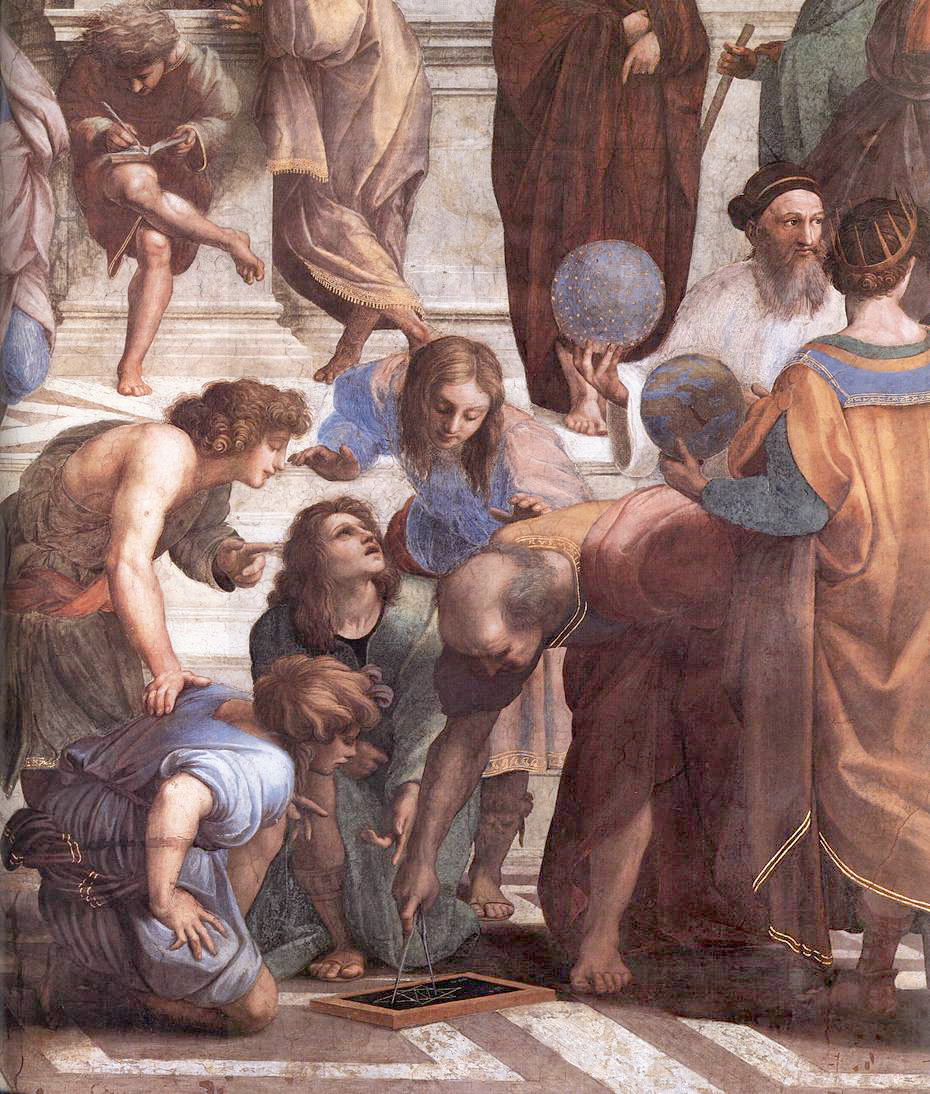
\includegraphics[scale=0.6]{pics/greece.jpg}
    \end{figure}
    %
\end{columns}
\end{frame}
%%%%%%%%%%%%%%%%%%%%%%%%%%%%%%%%%%%%%%
\usebackgroundtemplate{%
\tikz[overlay,remember picture] \node[opacity=0.3, at=(current page.center)] {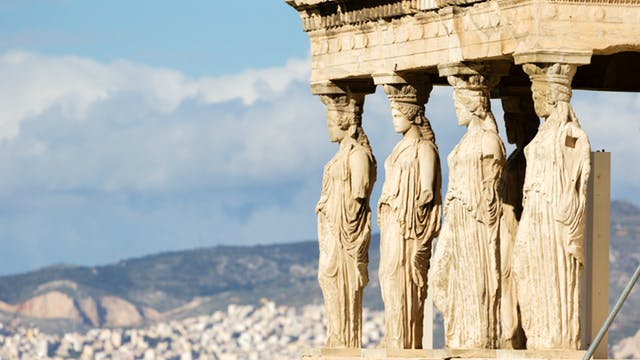
\includegraphics[height=\paperheight,width=\paperwidth]{pics/back.jpg}};
}
%%%%%%%%%%%%%%%%%%%%%%%%%%%%%%%%%%%%%%%
%        SLIDE 
%%%%%%%%%%%%%%%%%%%%%%%%%%%%%%%%%%%%%%%
\subsection{Why should we learn Geometry?}
\begin{frame}{Why should we learn Geometry?}
\begin{itemize}    
    \item Daily life: Brain Calculation, Installing wallpaper, Any measurement at house, Parallel parking, and so on.
    \item Nowadays we used Geometry in: 
        \begin{itemize}    
            \item Arts
            \item Astronomy
            \item Engineering
            \item Drafting
            \item Geology
            \item Architecture
            \item $\ \vdots$
        \end{itemize}
    \item Helpful for: 
        \begin{itemize}
            \item Improving analyzing skills
            \item problem-solving skills
            \item deductive reasoning
            \item $\ \vdots$
        \end{itemize}
\end{itemize}

\end{frame}
%%%%%%%%%%%%%%%%%%%%%%%%%%%%%%%%%%%%%%
\usebackgroundtemplate{ }% undeclare it
%%%%%%%%%%%%%%%%%%%%%%%%%%%%%%%%%%%%%%%
%        SLIDE 
%%%%%%%%%%%%%%%%%%%%%%%%%%%%%%%%%%%%%%%
\section{Different Types of Geometries}
\begin{frame}{Different Types of Geometries}
    \begin{figure}[H]
        \centering
        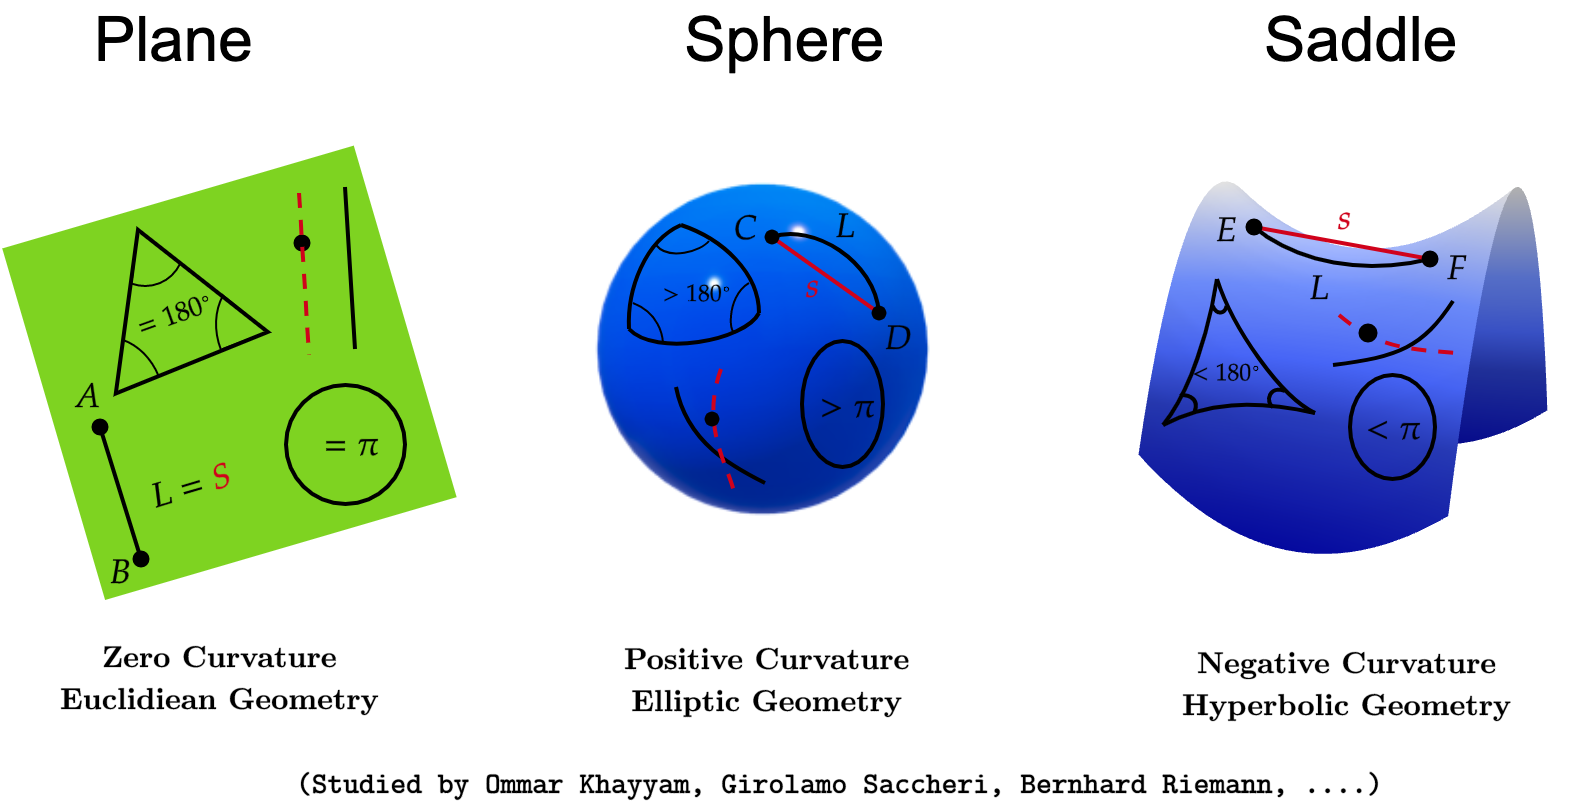
\includegraphics[width=0.8\textwidth]{pics/Euclid_vs_non_Euclid.png}
    \end{figure}
\end{frame}
%%%%%%%%%%%%%%%%%%%%%%%%%%%%%%%%%%%%%%%
%        SLIDE 
%%%%%%%%%%%%%%%%%%%%%%%%%%%%%%%%%%%%%%%
\section{Lines}
\begin{frame}{Lines}
    \begin{block}{Definition}
    \begin{itemize}
        \item  A line is a set of points (points are labeled with capital letters). 
        \item  In other words, a line is
        \setbeamertemplate{items}[triangle]
                    \begin{itemize}
                        \item straight (no bends)
                        \item and extend in both directions without end (infinitely)
                    \end{itemize}
        \setbeamertemplate{items}[default]
    \end{itemize}
    \end{block}
    %
    \begin{figure}[H]
        \centering
        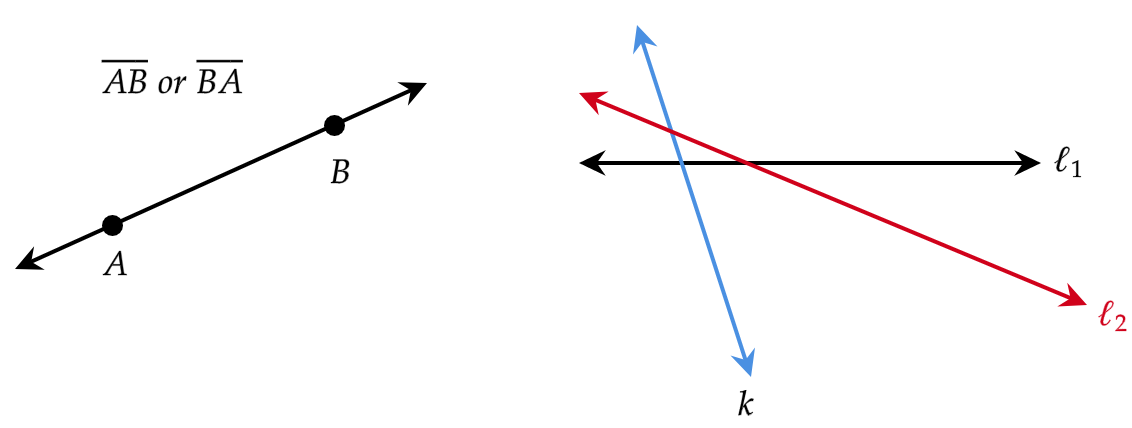
\includegraphics[scale=0.25]{pics/lines.png}
    \end{figure}
\end{frame}
%%%%%%%%%%%%%%%%%%%%%%%%%%%%%%%%%%%%%%%
%        SLIDE 
%%%%%%%%%%%%%%%%%%%%%%%%%%%%%%%%%%%%%%%
\subsection{Parallel Lines}
\begin{frame}{Parallel Lines}
    \begin{itemize}
        \item Lines are parallel if they are always the same distance apart and will never meet.
    \end{itemize}
    %
    \begin{figure}[H]
        \centering
        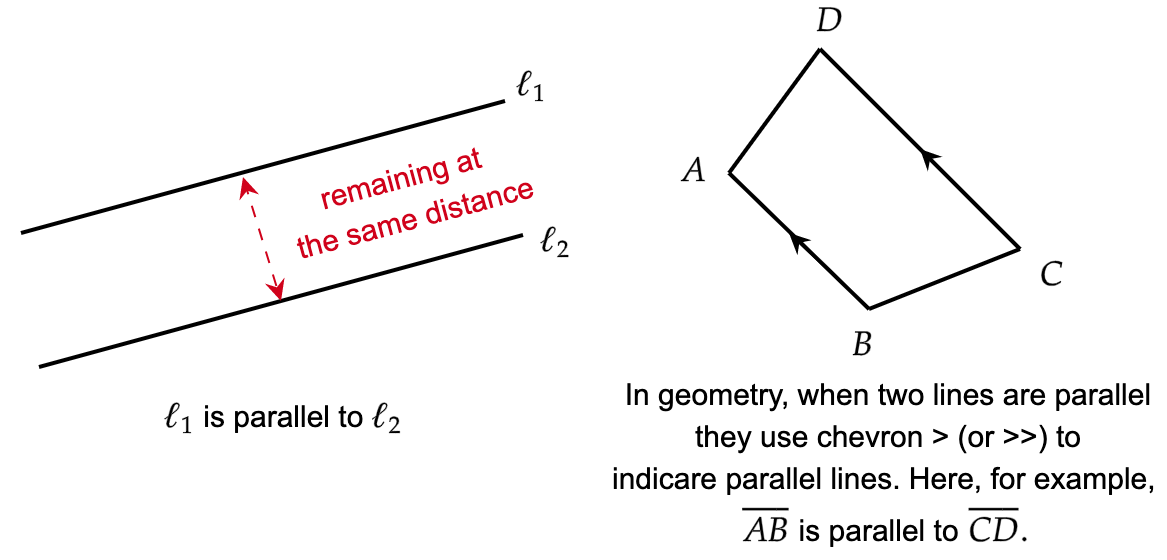
\includegraphics[scale=0.3]{pics/parallel_lines.png}
    \end{figure}
\end{frame}
%%%%%%%%%%%%%%%%%%%%%%%%%%%%%%%%%%%%%%%
%        SLIDE 
%%%%%%%%%%%%%%%%%%%%%%%%%%%%%%%%%%%%%%%
\subsection{Ray}
\begin{frame}{Ray}
    \begin{itemize}
        \item A part of a line that has one endpoint and goes on infinitely in one direction.
        \item A ray can be named using its endpoint first and then any other point on the ray.
    \end{itemize}
    %
    \begin{figure}[H]
        \centering
        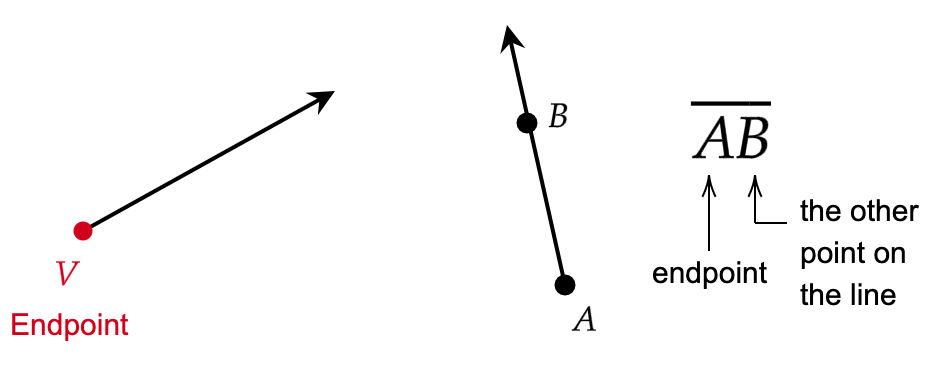
\includegraphics[scale=0.35]{pics/ray.png}
    \end{figure}
\end{frame}
%%%%%%%%%%%%%%%%%%%%%%%%%%%%%%%%%%%%%%%
%        SLIDE 
%%%%%%%%%%%%%%%%%%%%%%%%%%%%%%%%%%%%%%%
\section{Planes}
\begin{frame}[t]{Planes}
    \begin{columns}[c]
    \column{0.5\textwidth}
    \begin{block}{Definition}
    \begin{itemize}
        \item A plane is a two-dimensional surface that extends infinitely in both directions, like an infinitely large white board.
    \end{itemize}
    \end{block}
    %
    \footnotesize{
    \textbf{Some Properties of Planes}
    \begin{itemize}
        \item Any three points that are not on the same line (noncollinear points) determine a unique plane.
        \item The intersection of two distinct planes is a line.
        \item Any line and a point not on the line determine a unique plane.
        \item A line in a plane divides the plane into three parts, the line itself and two half planes.
        \item Two planes that do not intersect are said to be \textit{parallel planes}.
    \end{itemize}}
    %
    \column{0.45\textwidth}
    \begin{figure}
        \centering
        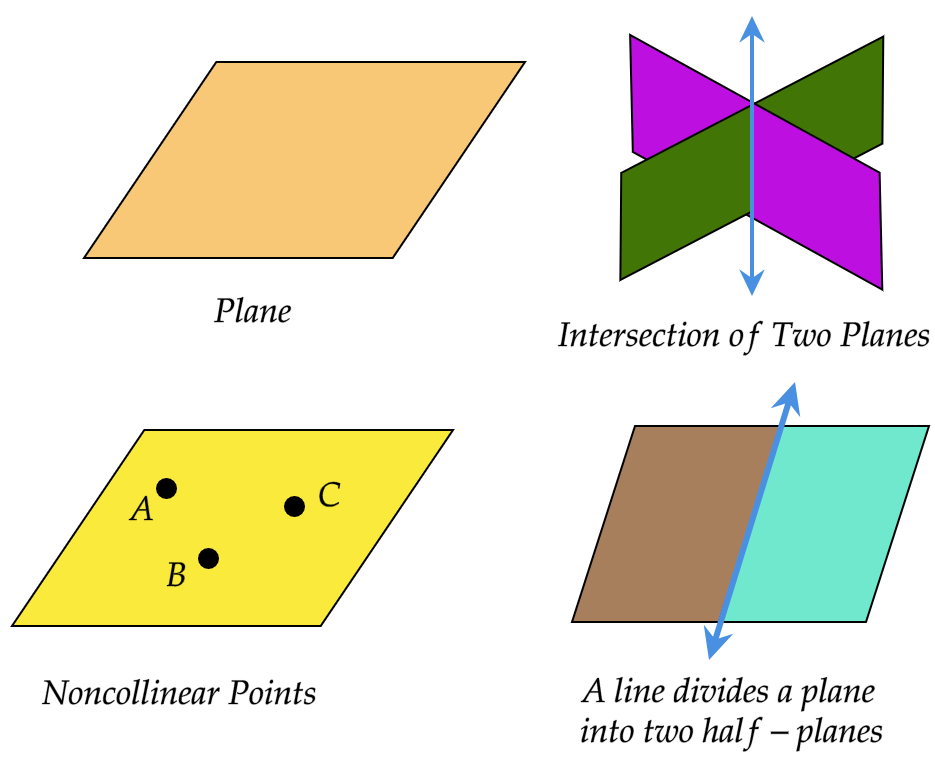
\includegraphics[scale=0.18]{pics/planes.png}
    \end{figure}
    \end{columns}
\end{frame}
%%%%%%%%%%%%%%%%%%%%%%%%%%%%%%%%%%%%%%%
%        SLIDE 
%%%%%%%%%%%%%%%%%%%%%%%%%%%%%%%%%%%%%%%
\section{Angles}
\begin{frame}[t]{Angles}
    \begin{block}{Definition}
    \begin{itemize}
        \item Two rays with a common endpoint form an angle.
        \item The common end point is called vertex.
        \item An angle is the amount of rotation from one ray to the other ray.
        \item Angle is denoted as $\angle $
    \end{itemize}
    \end{block}
    %
    \begin{figure}[H]
    \centering
    \usetikzlibrary{quotes,angles}
    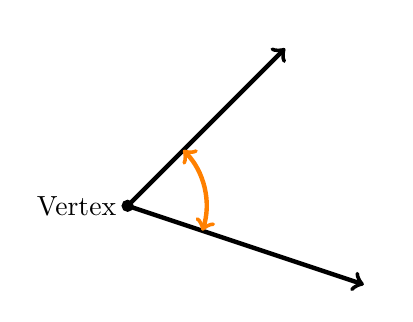
\begin{tikzpicture}
      \fill[black] (0,0)  circle[radius=2pt]; 
      \draw (0,0)  circle[radius=2pt]; 
      %
      \draw[ultra thick,<->]
        (3,-1) coordinate (a) node[right] {}
        -- (0,0) coordinate (b) node[left] {Vertex}
        -- (2,2) coordinate (c) node[above right] {}
        pic[draw=orange, ultra thick, <->, angle eccentricity=1.2, angle radius=1cm]
        {angle=a--b--c};
    \end{tikzpicture}
    \end{figure}
\end{frame}
%%%%%%%%%%%%%%%%%%%%%%%%%%%%%%%%%%%%%%%
%        SLIDE 
%%%%%%%%%%%%%%%%%%%%%%%%%%%%%%%%%%%%%%%
\subsection{How to Name an Angle?}
\begin{frame}[t]{How to Name an Angle?}
    Angles can be named in 3 ways:
    \small{
    \begin{enumerate}
        \item \textbf{Point-Vertex-Point}: The angle is names from a point on one ray, the vertex, and a point on the other ray. This is the most common way to name an angle.
        \item \textbf{Vertex method}: In case where it is not ambiguous, an angle can be named based solely on its vertex.
        \item \textbf{Number or Letter}: We can also use a lower-case letter or Greek letter or just a number to simply call an angle.
    \end{enumerate}}
    %
    \begin{figure}[H]
        \centering
        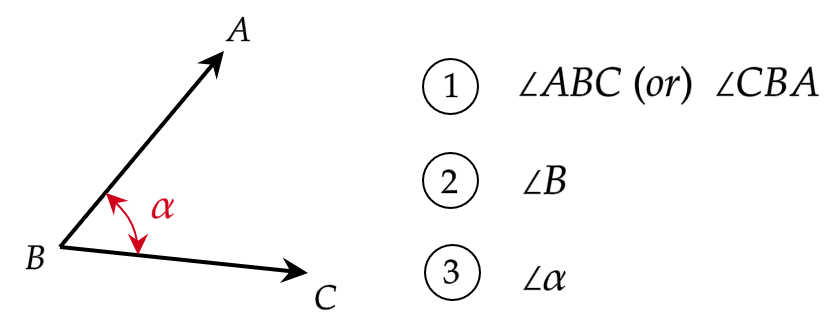
\includegraphics[scale=0.28]{pics/name_angles.png}
    \end{figure}
\end{frame}
%%%%%%%%%%%%%%%%%%%%%%%%%%%%%%%%%%%%%%%
%        SLIDE 
%%%%%%%%%%%%%%%%%%%%%%%%%%%%%%%%%%%%%%%
\section{Measure of Angles}
\begin{frame}[t]{Measure of Angles}
    \begin{itemize}
        \item The amount of rotation from one side to other is the measure of an angle.
        \item Angles can be measure in degrees, radians, or gradients.
        \item A protractor is used to measure angles.
        \item Let's discuss degrees and radians (most common ones).
    \end{itemize}
    %
    \begin{figure}[H]
        \centering
        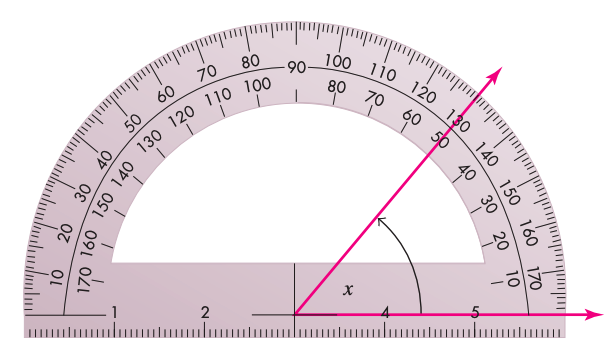
\includegraphics[scale=0.3]{pics/protractor.png}
        \caption*{Can you tell the measure of angle $\angle x$?}
    \end{figure}
\end{frame}
%%%%%%%%%%%%%%%%%%%%%%%%%%%%%%%%%%%%%%%
%        SLIDE 
%%%%%%%%%%%%%%%%%%%%%%%%%%%%%%%%%%%%%%%
\subsection{Degrees vs Radians}
\begin{frame}[t]{Degrees vs Radians}
    \begin{columns}[t]
    %1st
    \column{0.45\textwidth}
    \textbf{Degrees}
        \begin{itemize}
            \item We use $^\circ$ to denote an angle in degree.
            \item Here, full rotation is $360^\circ$.
            \item So if we divide a circle into equally $360$ parts, each part is $1^\circ$.
        \end{itemize}
        %
        \begin{figure}[H]
            \centering
            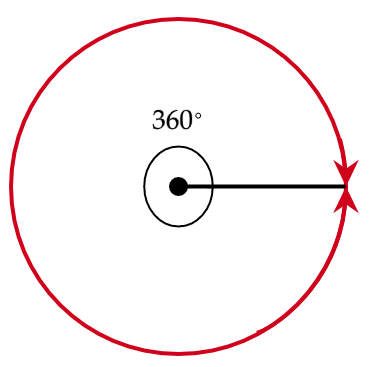
\includegraphics[width=0.45\textwidth]{pics/degrees.png}
        \end{figure}
    %2nd
    \column{0.45\textwidth}
    \textbf{Radians}
        \begin{itemize}
            \item It is a pure measure based on the Radius of the circle.
            \item If the arc between two points is equal to radius (R), corresponding angle is 1 radian. So, full rotation is $2\pi$.
        \end{itemize}
        %
        \vspace{0.5em}
        \begin{figure}[H]
            \centering
            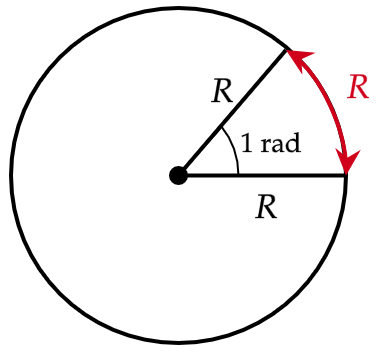
\includegraphics[width=0.45\textwidth]{pics/radians.png}
        \end{figure}
    \end{columns}
\end{frame}
%%%%%%%%%%%%%%%%%%%%%%%%%%%%%%%%%%%%%%%
%        SLIDE 
%%%%%%%%%%%%%%%%%%%%%%%%%%%%%%%%%%%%%%%
\subsection{Common Angles}
\begin{frame}{Common Angles}
    \begin{figure}[H]
        \centering
        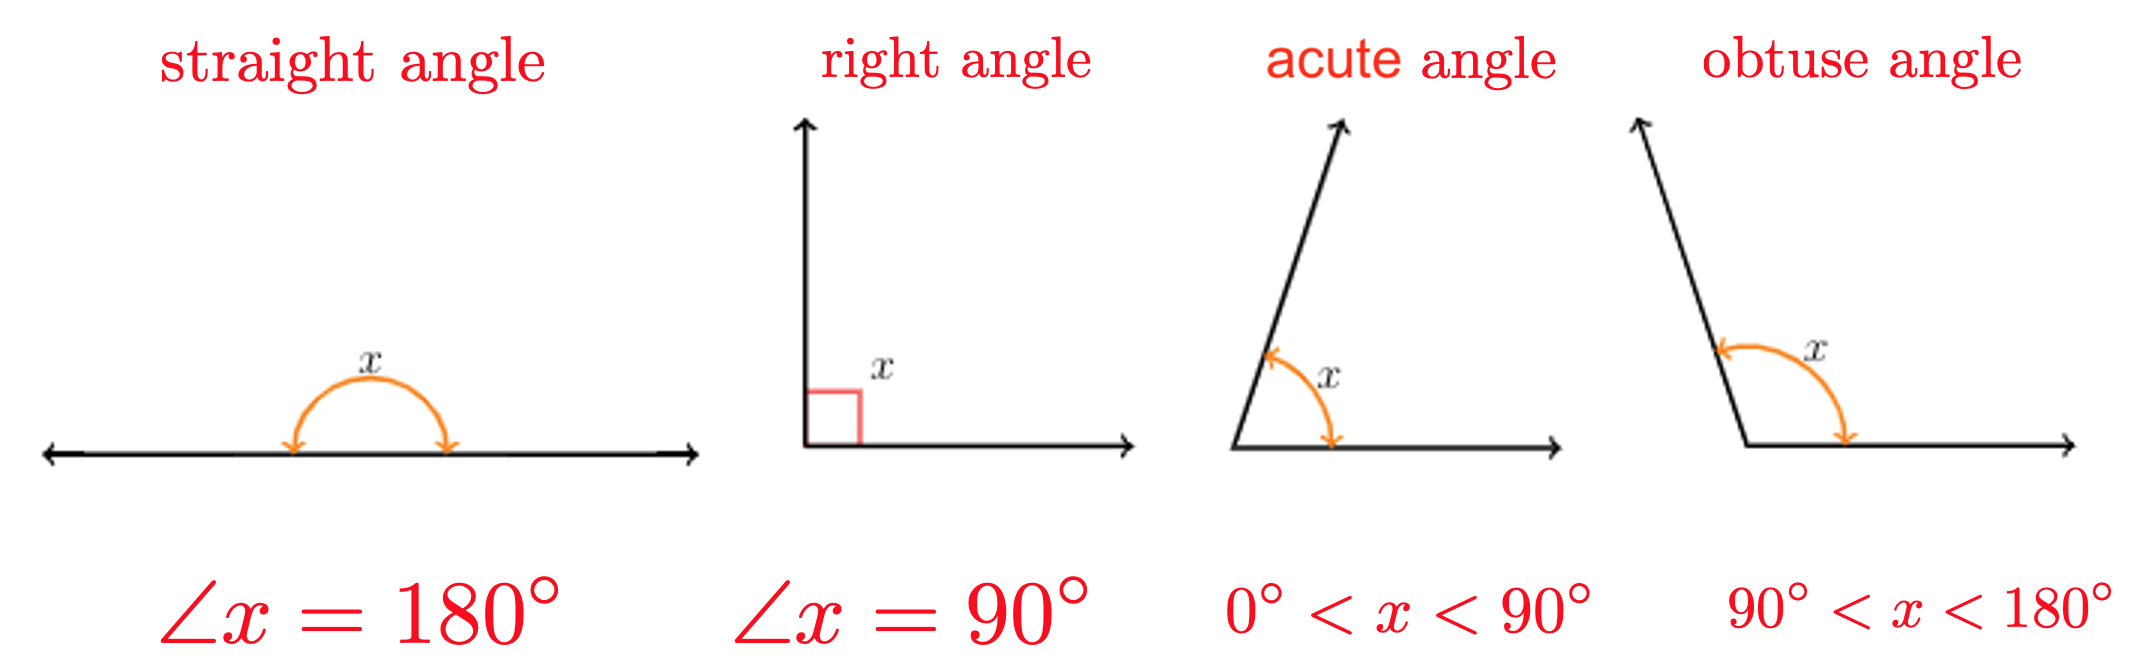
\includegraphics[scale=0.4]{pics/common_angles.png}
    \end{figure}
\end{frame}
%%%%%%%%%%%%%%%%%%%%%%%%%%%%%%%%%%%%%%%
%        SLIDE 
%%%%%%%%%%%%%%%%%%%%%%%%%%%%%%%%%%%%%%%
\addtocontents{toc}{\newpage}
%%%%%%%%%%%%%%%%%%%%%%%%%%%%%%%%%%%%%%%
\section{Important Angles}
\subsection{Adjacent Angles}
\begin{frame}{Adjacent Angles}
    \begin{block}{Definition}
        Angles that have \textbf{a common vertex and a common side but do not overlap} are called adjacent angles.
    \end{block}
    %
    \begin{figure}[H]
        \centering
        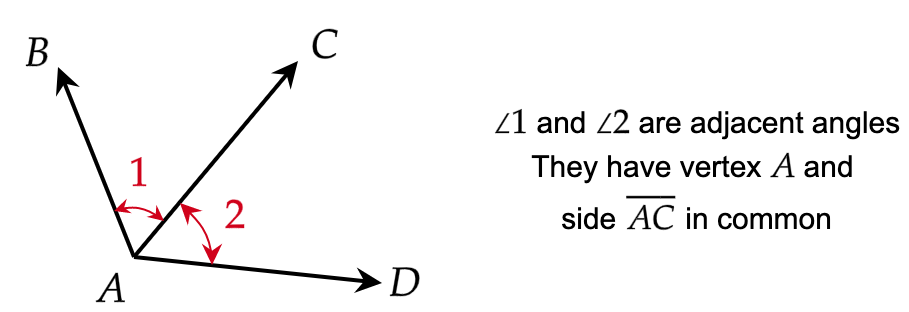
\includegraphics[scale=0.3]{pics/adjacent.png}
    \end{figure}
\end{frame}
%%%%%%%%%%%%%%%%%%%%%%%%%%%%%%%%%%%%%%%
%        SLIDE 
%%%%%%%%%%%%%%%%%%%%%%%%%%%%%%%%%%%%%%%
\subsection{Supplementary Angles}
\begin{frame}[t]{Supplementary and Complementary Angles}
    \begin{columns}
    %
    \column{0.42\textwidth}
    \begin{block}{Supplementary Angles}
        If two angles add up to $180^\circ$, then they are supplementary angles.
    \end{block}
    %
    \begin{figure}[H]
        \centering
        \usetikzlibrary{quotes,angles}
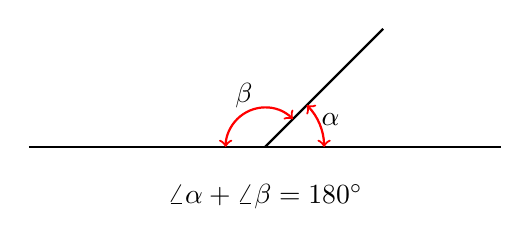
\begin{tikzpicture}[scale=1.5]
  %
  \coordinate (a) at (-2,0);
  \coordinate (o) at (0,0) node[below=1em] {$\angle \alpha + \angle \beta = 180^\circ$};
  \coordinate (c) at (1,1);
  \coordinate (d) at (2,0);
  %
  \draw[thick] (a) -- (o);
  \draw[thick] (o) -- (c);
  \draw[thick] (o) -- (d);
  %
  \draw pic["$\alpha$", thick, draw=red, <->, angle eccentricity=1.2, angle radius=0.75cm] {angle=d--o--c};
   \draw pic["$\beta$", thick, draw=red, <->, angle eccentricity=1.4, angle radius=0.5cm] {angle=c--o--a};
   
\end{tikzpicture}
    \end{figure}
    %
    \column{0.42\textwidth}
    \begin{block}{Complementary Angles}
        If two angles add up to $90^\circ$, then they are complementary angles.
    \end{block}
    %
    \begin{figure}[H]
        \centering
        \usetikzlibrary{quotes,angles}
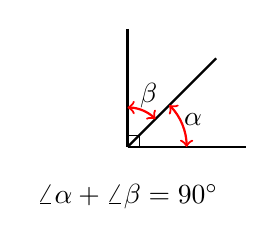
\begin{tikzpicture}[scale=1.5]
  %
  \coordinate (a) at (0,1);
  \coordinate (o) at (0,0) node[below=1em] {$\angle \alpha + \angle \beta = 90^\circ$};
  \coordinate (c) at (1,0);
  \coordinate (d) at (0.75,0.75);
  %
  \draw[thick] (a) -- (o);
  \draw[thick] (o) -- (c);
  \draw[thick] (o) -- (d);
  %
  \draw pic["$\alpha$", thick, draw=red, <->, angle eccentricity=1.2, angle radius=0.75cm] {angle=c--o--d};
   \draw pic["$\beta$", thick, draw=red, <->, angle eccentricity=1.4, angle radius=0.5cm] {angle=d--o--a};
   %
   \draw (o) -- (0,0.1) -- (0.1,0.1) -- (0.1,0);
\end{tikzpicture}
    \end{figure}
    %    
    \end{columns}
\end{frame}
%%%%%%%%%%%%%%%%%%%%%%%%%%%%%%%%%%%%%%%
%        SLIDE 
%%%%%%%%%%%%%%%%%%%%%%%%%%%%%%%%%%%%%%%
\subsection{Vertical Angles}
\begin{frame}[t]{Vertical Angles}
    \begin{block}{Definition}
        \begin{itemize}
            \item When two straight lines intersect, the non-adjacent angles
		    are called vertical angles.
		    \item Vertical angles are equal.
        \end{itemize}
    \end{block}
    %
    \begin{columns}
    \column{0.45\textwidth}
    Opposite angles are vertical angles. So,
    \begin{align*}
         \angle 1 &= \angle 3
         \\
         \angle 2 &= \angle 4
    \end{align*}
    %
    \column{0.45\textwidth}
    \begin{figure}[H]
        \centering
        \usetikzlibrary{quotes,angles}
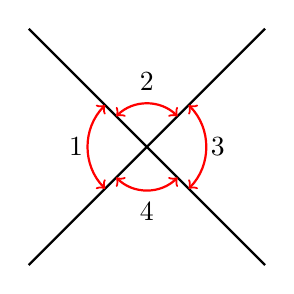
\begin{tikzpicture}[scale=1.5]
  %
  \coordinate (a) at (-1,1);
  \coordinate (o) at (0,0) ;
  \coordinate (b) at (1,-1);
  \coordinate (d) at (1,1);
  \coordinate (e) at (-1,-1);
  %
  \draw[thick] (a) -- (b);
  \draw[thick] (e) -- (d);
  %
   \draw pic["$1$", thick, draw=red, <->, angle eccentricity=1.2, angle radius=0.75cm] {angle=a--o--e};
   \draw pic["$2$", thick, draw=red, <->, angle eccentricity=1.5, angle radius=0.55cm] {angle=d--o--a};
   \draw pic["$3$", thick, draw=red, <->, angle eccentricity=1.2, angle radius=0.75cm] {angle=b--o--d};
   \draw pic["$4$", thick, draw=red, <->, angle eccentricity=1.5, angle radius=0.55cm] {angle=e--o--b};
   %
\end{tikzpicture}
    \end{figure}  
          %
    \end{columns}
\end{frame}
%%%%%%%%%%%%%%%%%%%%%%%%%%%%%%%%%%%%%%%
%        SLIDE 
%%%%%%%%%%%%%%%%%%%%%%%%%%%%%%%%%%%%%%%
\begin{frame}[t]{Example (Find Missing Angles)}
    \begin{example}
    \begin{columns}[t]
    \column{0.7\textwidth}
     \small{$\angle CBA$ is equal to $20^\circ$.}
     \begin{enumerate}[(a)]
         \item \small{If $\angle DBC$ and $\angle CBA$ are complementary angles, find $\angle DBC$.}
         \item \small{If $\angle CBA$ and $\angle CBE$ are supplementary angles, find $\angle DBE$.}
     \end{enumerate}
     %
     \column{0.3\textwidth}
     \begin{figure}[H]
         \centering
         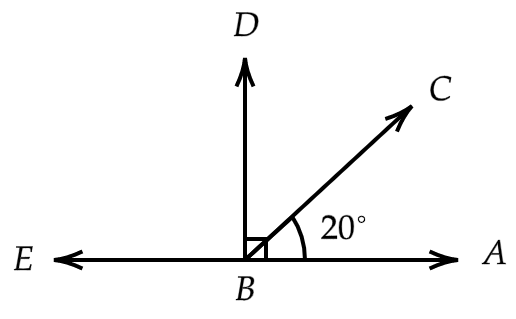
\includegraphics[scale=0.25]{pics/example_1.png}
     \end{figure}
     \end{columns}
    \end{example}
\end{frame}
%%%%%%%%%%%%%%%%%%%%%%%%%%%%%%%%%%%%%%%
%        SLIDE 
%%%%%%%%%%%%%%%%%%%%%%%%%%%%%%%%%%%%%%%
\section{Transversal Line}
\begin{frame}{Transversal Line}
    \begin{block}{Definition}
        \begin{itemize}
            \item A transversal line is a line that intersects two different lines at different points.
            \item A transveral line forms eight angles.
        \end{itemize}
    \end{block}
    %
    \begin{figure}[H]
        \centering
        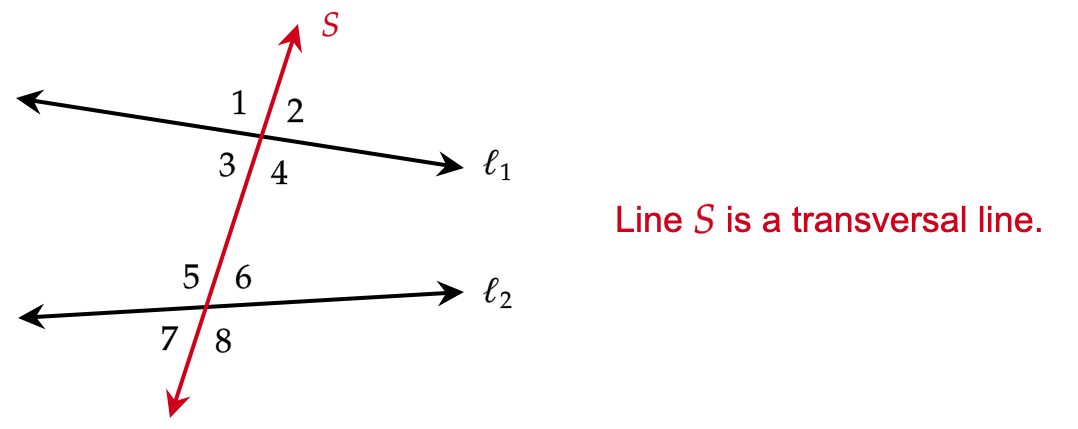
\includegraphics[scale=0.3]{pics/transversal_line.png}
    \end{figure}
\end{frame}
%%%%%%%%%%%%%%%%%%%%%%%%%%%%%%%%%%%%%%%
%        SLIDE 
%%%%%%%%%%%%%%%%%%%%%%%%%%%%%%%%%%%%%%%
\subsection{Interior and Exterior Angles}
\begin{frame}[t]{Interior and Exterior Angles}
    \begin{columns}
    \column{0.45\textwidth}
    %
    \textbf{Interior Angles}
    \begin{itemize}
        \item Angles that are form inside $\ell_1$ and $\ell_2$ are called \textit{interior angles}.
    \end{itemize}
    %
    %
    \begin{figure}[H]
        \centering
        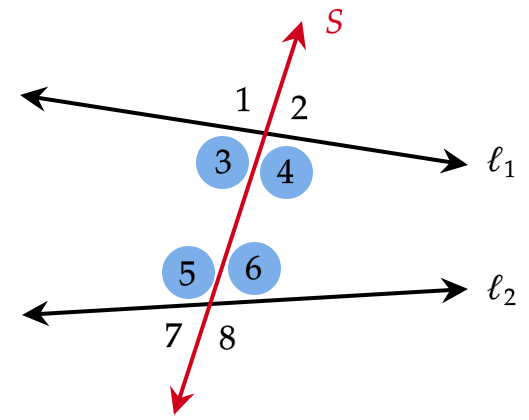
\includegraphics[scale=0.3]{pics/interior_angles.png}
    \end{figure}    
    \column{0.45\textwidth}
    %
    \textbf{Exterior Angles}
    \begin{itemize}
        \item Angles that are form outside $\ell_1$ and $\ell_2$ are called \textit{exterior angles}.
    \end{itemize}
    %    
    \begin{figure}[H]
        \centering
        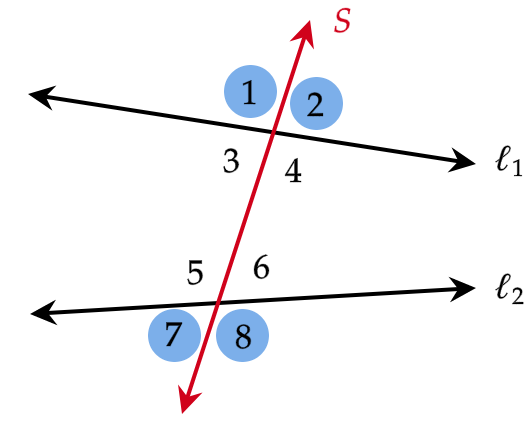
\includegraphics[scale=0.3]{pics/exterior_angles.png}
    \end{figure} 
    \end{columns}
\end{frame}
%%%%%%%%%%%%%%%%%%%%%%%%%%%%%%%%%%%%%%%
%        SLIDE 
%%%%%%%%%%%%%%%%%%%%%%%%%%%%%%%%%%%%%%%
\subsection{Corresponding Angles}
\begin{frame}{Corresponding Angles}
    \begin{itemize}
        \item one exterior angle and one interior angle on the same side of transversal line are called \textit{corresponding angles} for these lines.
    \end{itemize}
    %
    \begin{figure}[H]
        \centering
        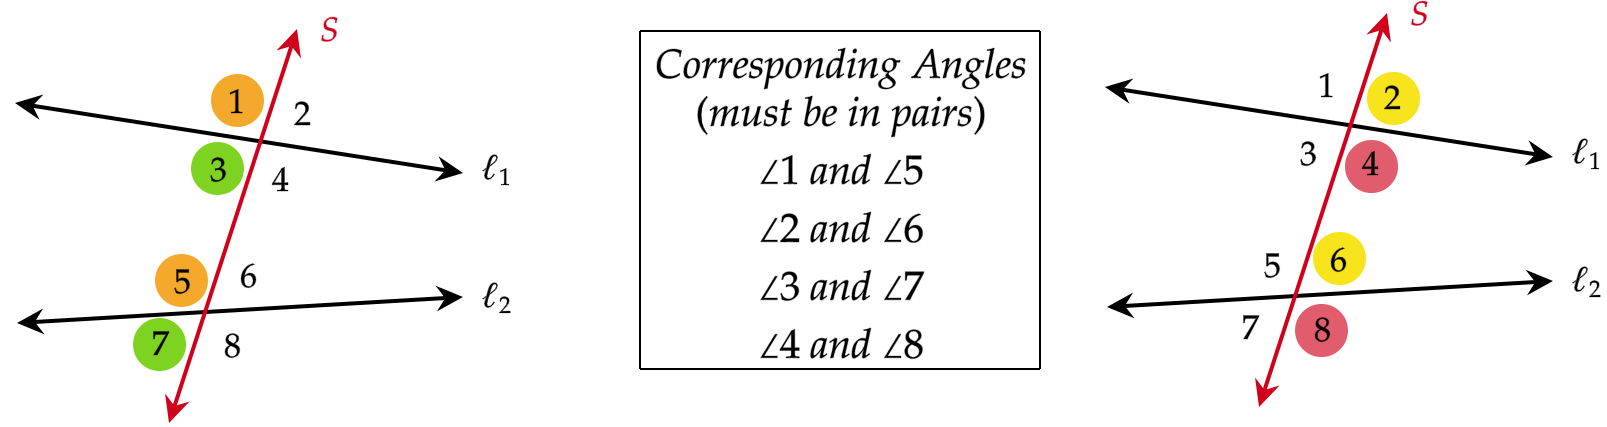
\includegraphics[scale=0.25]{pics/corresponding.png}
    \end{figure}
\end{frame}
%%%%%%%%%%%%%%%%%%%%%%%%%%%%%%%%%%%%%%%
%        SLIDE 
%%%%%%%%%%%%%%%%%%%%%%%%%%%%%%%%%%%%%%%
\subsection{Alternate Interior Angles}
\begin{frame}{Alternate Interior Angles}
    \begin{itemize}
        \item Two interior angles that have different vertices and lie on opposite sides of the transversal are \textit{alternate interior angles}.
    \end{itemize}
    %
    \begin{figure}[H]
        \centering
        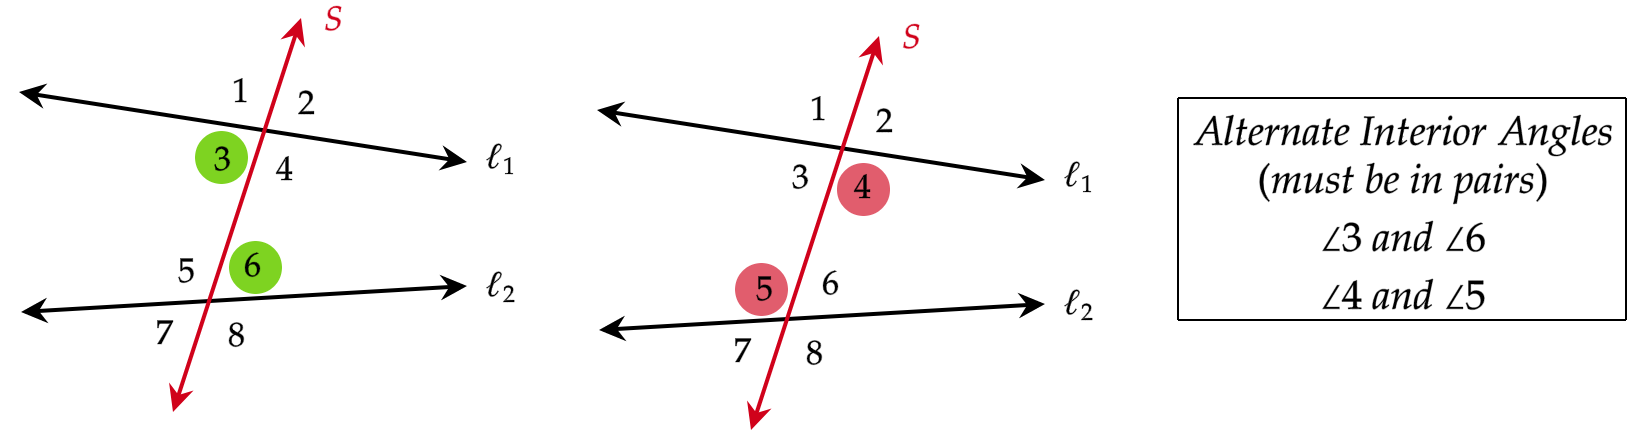
\includegraphics[scale=0.25]{pics/alternate_interior_angles.png}
    \end{figure}
\end{frame}
%%%%%%%%%%%%%%%%%%%%%%%%%%%%%%%%%%%%%%%
%        SLIDE 
%%%%%%%%%%%%%%%%%%%%%%%%%%%%%%%%%%%%%%%
\subsection{Alternate Exterior Angles}
\begin{frame}{Alternate Exterior Angles}
    \begin{itemize}
        \item Two exterior angles that have different vertices and lie on opposite sides of the transversal are \textit{alternate exterior angles}.
    \end{itemize}
    %
    \begin{figure}[H]
        \centering
        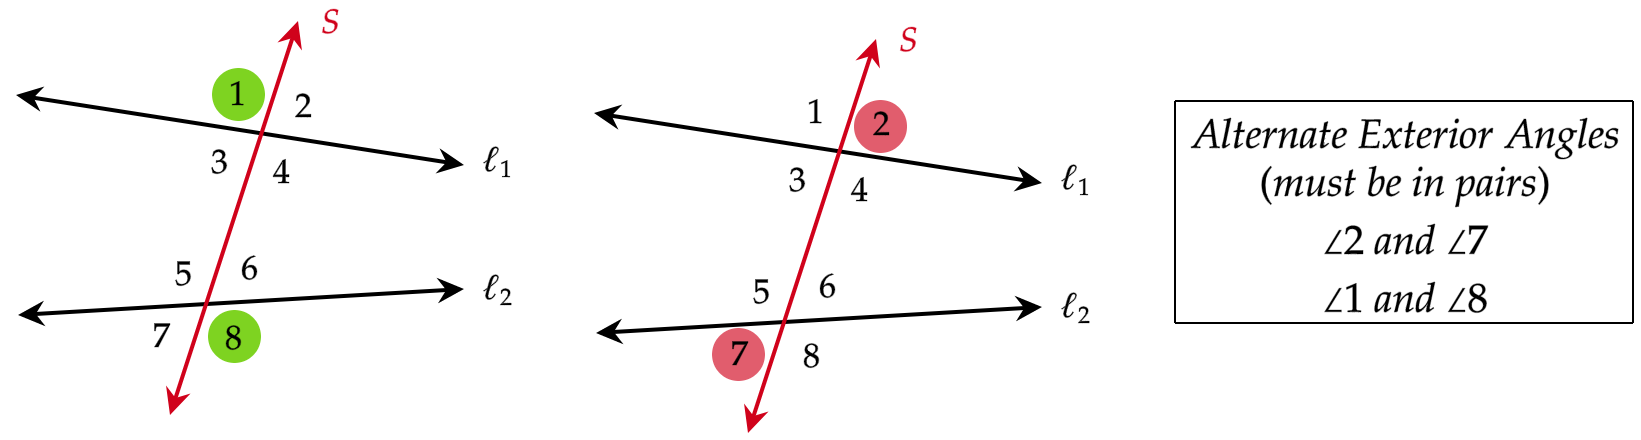
\includegraphics[scale=0.25]{pics/alternate_exterior_angles.png}
    \end{figure}
\end{frame}
%%%%%%%%%%%%%%%%%%%%%%%%%%%%%%%%%%%%%%%
%        SLIDE 
%%%%%%%%%%%%%%%%%%%%%%%%%%%%%%%%%%%%%%%
\section{Parallel lines and a Transversal Line}
\begin{frame}{Parallel lines and a Transversal Line}
    \begin{itemize}
        \item If a transversal line intersects two parallel lines, then
    \end{itemize}
    \begin{figure}[H]
        \centering
        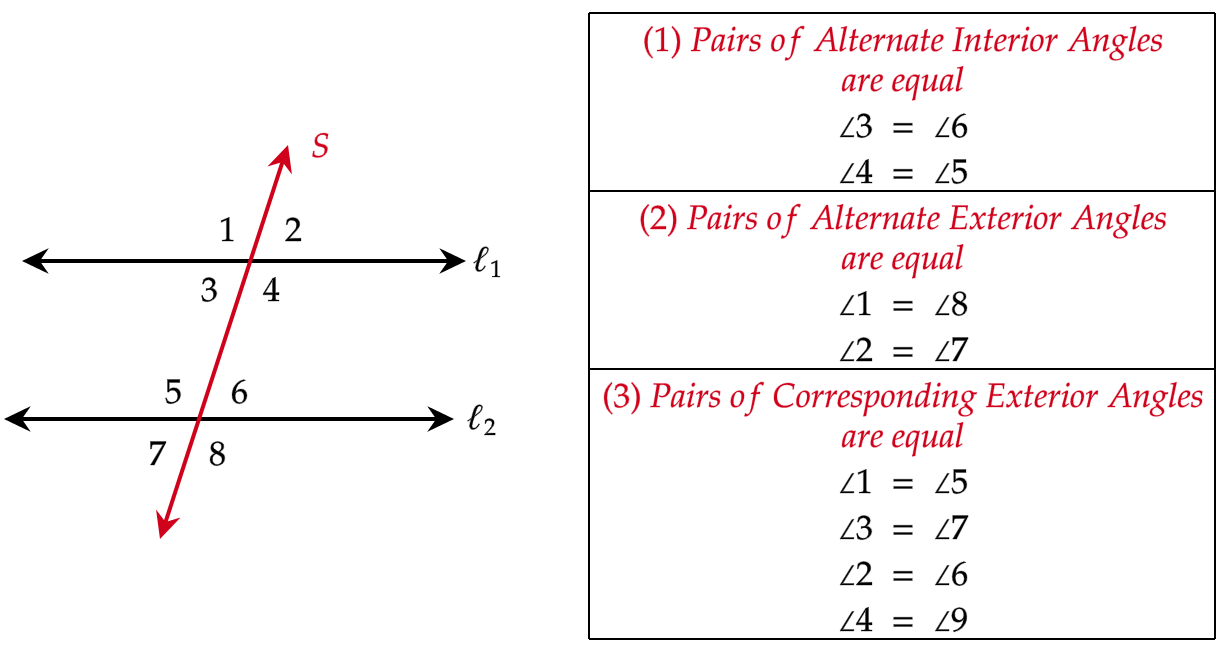
\includegraphics[scale=0.28]{pics/parallel_transversal.png}
    \end{figure}
\end{frame}
%%%%%%%%%%%%%%%%%%%%%%%%%%%%%%%%%%%%%%%
%        SLIDE 
%%%%%%%%%%%%%%%%%%%%%%%%%%%%%%%%%%%%%%%
\subsection{Summary}
\begin{frame}{Summary}
    \begin{figure}[H]
        \centering
        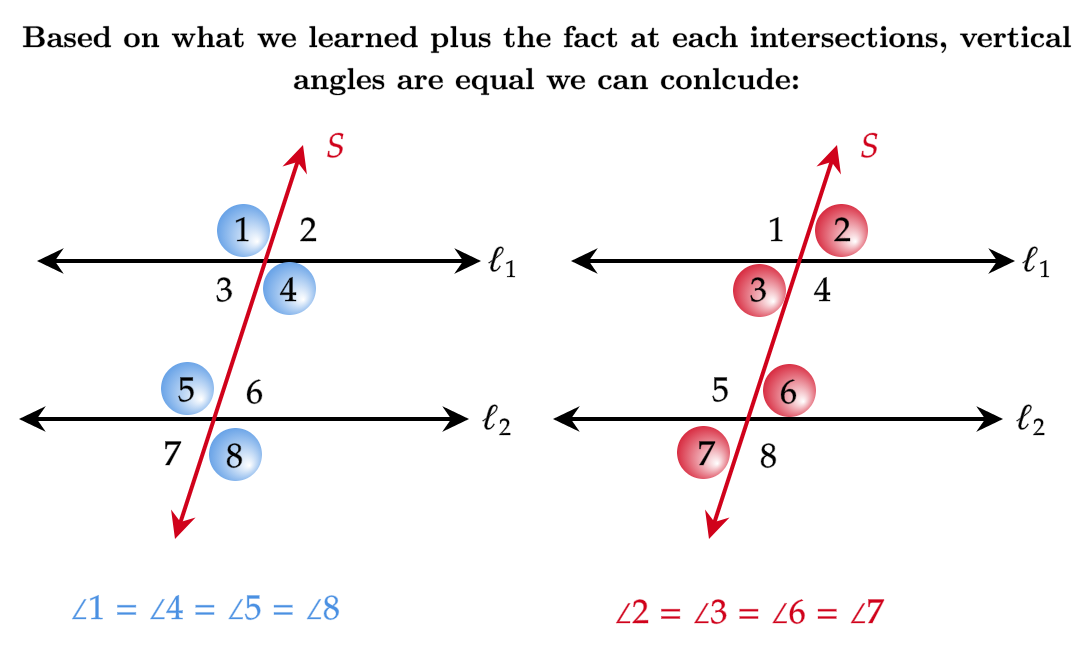
\includegraphics[scale=0.3]{pics/summaray_parallel.png}
    \end{figure}
\end{frame}
%%%%%%%%%%%%%%%%%%%%%%%%%%%%%%%%%%%%%%%
%        SLIDE 
%%%%%%%%%%%%%%%%%%%%%%%%%%%%%%%%%%%%%%%
\begin{frame}[t]{Example (Parallel Lines)}
    \begin{example}
        \begin{columns}[t]
        \column{0.45\textwidth}
        In figure below, line $\ell$ is parallel to line $m$ and $\angle 2 =117^\circ$. Determine all remaining angles.
        %
        \column{0.45\textwidth}
        \begin{figure}[H]
            \centering
            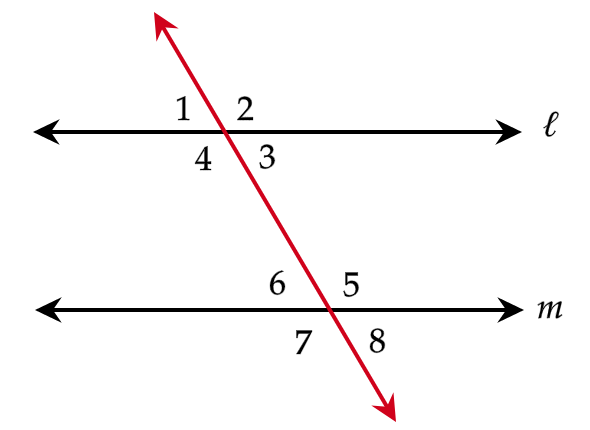
\includegraphics[scale=0.2]{pics/parallel_example.png}
        \end{figure}
        \end{columns}
    \end{example}
\end{frame}